% !TEX TS-program = pdflatexmk
\documentclass[12pt]{amsart}
\usepackage{multicol}
\usepackage{float}

%\usepackage[parfill]{parskip}    % Activate to begin paragraphs with an empty line rather than an indent

\usepackage[margin=1in]{geometry}


\usepackage{amsmath,amssymb,amsthm,latexsym,graphicx}
\usepackage[normalem]{ulem}
\usepackage{setspace} %used for doublespacing, etc.
\usepackage{hyperref}
\usepackage{cancel}
\usepackage[dvipsnames,usenames]{color}
\usepackage[all]{xy}
\usepackage{fancyhdr}
\pagestyle{fancy}
	\renewcommand{\headrulewidth}{0.5pt} % and the line
	\headsep=1cm
	
\DeclareGraphicsRule{.tif}{png}{.png}{`convert #1 `dirname #1`/`basename #1 .tif`.png}

%Some useful environments.
\newtheorem{theorem}{Theorem}
\newtheorem{corollary}[theorem]{Corollary}
\newtheorem{conjecture}[theorem]{Conjecture}
\newtheorem{lemma}[theorem]{Lemma}
\newtheorem{proposition}[theorem]{Proposition}
\newtheorem{definition}[theorem]{Definition}
\newtheorem{example}[theorem]{Example}
\newtheorem{axiom}{Axiom}
\theoremstyle{remark}
\newtheorem{remark}{Remark}
\newtheorem*{exercise}{Exercise}%[section]

%Some useful shortcuts for our favorite fields
\def\RR{\ensuremath{\mathbb R}} %Note, you can use these WITHOUT entering math mode
\def\NN{\ensuremath{\mathbb N}}
\def\ZZ{\ensuremath{\mathbb Z}}
\def\QQ{{\ensuremath\mathbb Q}}
\def\CC{\ensuremath{\mathbb C}}
\def\EE{{\ensuremath\mathbb E}}

%Some useful shortcuts for formatting lists
\newcommand{\bc}{\begin{center}}
\newcommand{\ec}{\end{center}}
\newcommand{\be}{\begin{enumerate}}
\newcommand{\ee}{\end{enumerate}}
\newcommand{\bi}{\begin{itemize}}
\newcommand{\ei}{\end{itemize}}

%Some useful shortcuts for formatting mathematical symbols
\newcommand{\ol}[1]{\overline{#1}}
\newcommand{\oimp}[1]{\overset{#1}{\iff}} %labeled iff symbol
\newcommand{\bv}[1]{\ensuremath{ \vec{\mathbf{#1}}} } %makes a vector.
\newcommand{\mc}[1]{\ensuremath{\mathcal{#1}}} %put something in caligraphic font
\newcommand{\mpg}[1]{\marginpar{ #1}} %to put comments in margins
\newcommand{\bsl}[1]{\texttt{\symbol{92}{\em #1}}} %for backslashes.
\newcommand{\normale}{\trianglelefteq}
\newcommand{\normal}{\triangleleft}

%Code for formatting the proofs a little nicer for submitted homework
\makeatletter
\renewenvironment{proof}[1][\proofname]{\par\doublespacing
  \pushQED{\qed}%
  \normalfont \topsep6\p@\@plus6\p@\relax
  \list{}{%
    \settowidth{\leftmargin}{\itshape\proofname:\hskip\labelsep}%
    \setlength{\labelwidth}{0pt}%
    \setlength{\itemindent}{-\leftmargin}%
  }%
  \item[\hskip\labelsep\itshape#1\@addpunct{:}]\ignorespaces
}{%
  \popQED\endlist\@endpefalse
  \singlespacing
}
\makeatother


%Commenting tools. You can ignore this stuff unless we're exchanging materials where I'm commenting in detail on how you are writing/using LaTeX.
\usepackage{soul}
\definecolor{highlight}{rgb}{1,0.6,0.6}
\sethlcolor{highlight}
\newcommand{\hlm}[1]{\colorbox{highlight}{$\displaystyle #1$}}
\newtheoremstyle{mycomment}{\topsep}{-0in}{\small \itshape \sffamily}{}{\small \itshape\sffamily}{:}{.5em}{}
\theoremstyle{mycomment}
\newtheorem*{acomment}{\color{BrickRed}{Comment}}
\newcommand{\com}[1]{{\color{OliveGreen}\begin{acomment}{#1} %#2 \color{black} 
\end{acomment}\noindent}}
%\newcommand{\com}[1]{{\color{BrickRed}{\\ Comment:}\color{OliveGreen}{#1} \\}}
\newcommand{\red}[1]{{\color{BrickRed} #1}}
\newcommand{\blue}[1]{{\color{MidnightBlue}#1}}
\newcommand{\green}[1]{{\color{OliveGreen}#1}}
\newcommand{\mwrong}[2]{\red{\cancel{#1}}\green{#2}}
\newcommand{\wrong}[2]{\red{\sout{#1}}\green{#2}}
\definecolor{OliveGreen}{rgb}{.3,.5,.2}
\definecolor{MidnightBlue}{rgb}{.3,.4,.6}
\newcommand{\pts}[1]{\hfill\blue{{#1}/5}}

\chead{MATH 631F}
\pagestyle{fancy}
%Modify these items:
\rhead{\emph{Stefano Fochesatto}}
\lhead{\emph{HW \#3 --- \today}}

\DeclareMathOperator{\lcm}{lcm}
\begin{document}

\thispagestyle{fancy}
\author{Coordinator: Coordinator's Name}

% 2.3 1-3, 5, 8, 9, 16, 23.
% 2.4 1, 2, 4.
% 2.5 5, 6a, 6c, 8, 9.
% 3.1 1, 3, 4, 5, 7, 22, 24, 28, 31, 35, 36.
% 




\section*{\textbf{Section 2.3}}


\begin{exercise}[\textbf{2.3.1}] Find all subgroups of $Z_{45} = <x>,$ giving a generator for each. Describe the containments between these subgroups. 
  \begin{proof}[Solution] Recall that by properties of finite cyclic groups since $|<x>| = n$ then for each integer divisor $a$ dividing $n$ there exists a unique 
    subgroup of $<x>$ order $a$ generated by $<x^d>$, where $d = \frac{n}{a}$. Furthermore we know that every subgroup of $<x>$ corresponds bijectively to the positive divisors of $n$.\\
    Enumerating the divisors of $45$, 
    \begin{equation*}
      1, 3, 5, 9, 15, 45
    \end{equation*}
    Each corresponding bijectively to the group generated by $<x^d>$, where $d = \frac{n}{a}$
    \begin{equation*}
      <x^{45}>, <x^{15}>, <x^{9}>,<x^{5}>, <x^{3}>, <x>
    \end{equation*}
    Note that since $3 \mid 9, 15$ and $5 \mid 15$ we get the following lattice diagram, 
    \begin{figure}[H]
      \begin{center}
        \caption{Lattice Diagram for $Z_{45} = <x>$}
        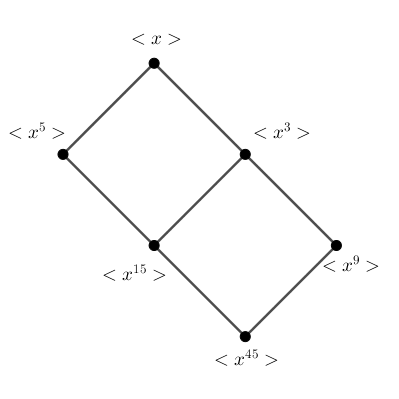
\includegraphics[width=.5\textwidth]{CyclicSubgroups.png}
      \end{center}
    \end{figure} 
    \end{proof}
\end{exercise}
\vspace{.15in}




\begin{exercise}[\textbf{2.3.2}] If $x$ is an element of the finite group $G$ and $|x| = |G|$, prove that $G = <x>$. Give an explicit example to show that this result 
  need not be true if $G$ is an infinite group.
  \begin{proof} Suppose $x$ is an element of the finite group $G$ such that $|x| = |G| = n$. Since $|x| = n$ we know that, $1, x, x^2, ../
    x^{n-1}$ are all distinct, since if there were two powers $x^j = x^i$ with $i < j < n$ then $x^{j - i} = 1$ and then $|x| \neq n$. Note that the 
    distinct powers $1, x, x^2, ../ x^{n-1}$, comprise $<x>$ we know that $<x>$ contains $n$ distinct elements, all powers of $x$ which must also be contained in $G$. Thus $<x> = G$.\\
    Consider the arithmetic group under $ZZ$, and let $x = 2$. The order of both $x$ and the set is infinite, however $<2>$ generates only positive integers.  
  \end{proof}
\end{exercise}
\vspace{.15in}




\begin{exercise}[\textbf{2.3.3}] Find all generators for $\ZZ/48\ZZ$. 
  \begin{proof}[Solutions:] By Proposition 6 we know that for some finite group $H$ with generator 
    $<x>$ whose order $|x| = n$ then $H = <x^a>$ if $(a, n) = 1$. Clearly $\ZZ/48\ZZ$ has generator
    generator $<\bar{1}>$ whose order is by definition $|<\bar{1}>| = 48$ Therefore all residue classes that generate 
    $\ZZ/48\ZZ$ are relatively prime to $48$. Therefore 
    $\overline{1}$, $   \overline{  5}$, $   \overline{  7}$, $   \overline{ 11}$, $   
    \overline{ 13}$, $   \overline{ 17}$, $   \overline{ 19}$, $   \overline{ 23}$, $   
    \overline{25}$, $   \overline{ 29}$, $   \overline{ 31}$, $   \overline{ 35}$, $   
    \overline{ 37}$, $   \overline{ 41}$, $   \overline{ 43}$, $   \overline{ 47}$
    Generate $\ZZ/48\ZZ$.
    \end{proof}
\end{exercise}
\vspace{.15in}


\begin{exercise}[\textbf{2.3.5}] Find the number of generators for $\ZZ/49000\ZZ$.
  \begin{proof}[Solution] As we recalled in the previous problem, every residual class whose representative is coprime to the 
    order of the group generates the the group. Using Euler's $\varphi-function$ we can find the number of elements from $[49000]$ which 
    are coprime to 49000. Determining the prime factorization of 49000, 
    \begin{equation*}
      49000 = 49(10^3) = (7^2)(5^3)(2^3)
    \end{equation*}
    Applying Euler's $\varphi-function$ we get, 
    \begin{equation*}
      \varphi(49000) = 7(6)5^2(4)2^2(1) = 16800.
    \end{equation*}
    \end{proof}
\end{exercise}
\vspace{.15in}


%%% Skipped 
\begin{exercise}[\textbf{2.3.8}] Let $Z_{48} = <x>$. For which integers $a$ does the map $\phi_a$ defined by $\phi_a :\overline{1} \to x^{a}$ extend to an 
  isomorphism from $\ZZ/48\ZZ$ into $\ZZ_{48}$.
  \begin{proof} 
    \end{proof}
\end{exercise}
\vspace{.15in}

%%% Skipped 
\begin{exercise}[\textbf{2.3.9}] Let $Z_{36} = <x>$ For which integers $a$ does the map $\phi_a$ defined by $\phi_a :\overline{1} \to x^{a}$ extend to a 
  well defined homomorphism from $\ZZ/48\ZZ$ into $\ZZ_{48}$.
  \begin{proof} 
    \end{proof}
\end{exercise}
\vspace{.15in}



\begin{exercise}[\textbf{2.3.16}] Assume $|x| = n$ and $|y| = m$. Suppose that $x$ and $y$ commute. Prove that $|xy|$
  divides the least common multiple of $m$ and $n$. Need this be true if $x$ and $y$ do not commute? Give an example of commuting elements $x, y$
  such that the order of $xy$ is not equal to the least common multiple of $|x|$ and $|y|$?
  \begin{proof} Let $|x| = n$ and $|y| = m$ and suppose that $x$ and $y$ commute. Let $i = \lcm(m,n)$, therefore there exists some $j, k \in \ZZ$ such that 
    $mj = i$ and $nk = i$. Since $x$ and $y$ commute, 
    \begin{equation*}
      (xy)^i = x^iy^i = x^{nk}y^{mj} = 1^k1^j = 1. 
    \end{equation*} 
    Since $(xy)^i = 1$ by Proposition 3 it follows that $|xy| \mid i$.
    For an example where commuting elements $x, y$ such that the order of $xy$ is not equal to the least common multiple of $|x|$ and $|y|$ consider the $\ZZ_4/\ZZ$
    and note that $|\overline{1}| = 4$ and $|\overline{3}| = 4$ and therefore the least common multiple is 4 but $|\overline{3}\overline{1}| = |\overline{4}| = 1 \neq 4$.
    \end{proof}
\end{exercise}
\vspace{.15in}


%% Probably wrong. 
\begin{exercise}[\textbf{2.3.23}] Show that $(\ZZ/2^n\ZZ)$ is not cyclic for any $n \geq 3$ [Find two distinct subgroups of order 2].
  \begin{proof} To show that $(\ZZ/2^n\ZZ)$ is not cyclic it is sufficient to show that $(\ZZ/2^n\ZZ)$ contains two distinct subgroups of order two. Meaning there are 
    two subgroups, $H, G$ of $(\ZZ/2^n\ZZ)$ with elements $H = {1, h}$ and $G = {1, g}$ such that $h \neq g$. This property demonstrates that
    there is no single $x \in (\ZZ/2^n\ZZ)$ for which $h, g \in <x>$ and therefore $(\ZZ/2^n\ZZ) \neq <x>$. Let $n \geq 3$, and consider
    $G = {1, 2^{n} + 1}$ and $H = {1, 2^{n} - 1}$. Note that, 
    \begin{equation*}
      gg = (2^{n - 1} + 1)^2 = (2^{n - 1}(2^{n - 1}) + (2)2^{n} + 1^2) = (2^{2n - 2} + (2)2^{n} + 1^2) = 2^{n}(2^{n}2^(-2) + 2) + 1 \cong 1 mod 2^n 
    \end{equation*}
    \begin{equation*}
      hh = (2^{n - 1} - 1)^2 = (2^{n - 1}(2^{n - 1}) - (2)2^{n} + 1^2) = (2^{2n - 2} - (2)2^{n} + 1^2) = 2^{n}(2^{n}2^(-2) - 2) + 1 \cong 1 mod 2^n 
    \end{equation*}
    Note that $2^{n - 1} + 1 \neq  2^{n - 1} - 1$ since $n \geq 3$ Therefore $H$ and $G$ are two distinct subgroups of order 2. Thus $(\ZZ/2^n\ZZ)$ is not cyclic.
  \end{proof}
\end{exercise}
\vspace{.15in}




%%% Also pretty bad. 
\section*{\textbf{Section 2.4}}
\begin{exercise}[\textbf{2.4.1}] Prove that if $H$ is a subgroup of $G$ then $<H> = H$. 
  \begin{proof} Suppose $H$ is a subgroup of $G$, and consider the subgroup of $G$ generated by the set $H$, $<H>$. By definition 
    \begin{equation*}
      <H> = \bigcap_{H \subseteq H and H \leq G} H. 
    \end{equation*}
    $<H>$ is the intersection of all subgroups of $G$ containing the set $H$. However $H$ is a subgroup, and therefore any subgroup of $G$ which contains an element from $H$
    must contain the whole set $H$. Thus intersection of all subgroups of $G$ containing the set $H$ is the group $H$. 
    \end{proof}
\end{exercise}
\vspace{.15in}


\begin{exercise}[\textbf{2.4.2}] Prove that if $A$ is a subset of $B$ then $<A> \leq <B>$. Give an example where $A \subset B$ with $A \neq B$ but $<A> = <B>$. 
  \begin{proof} Let $G$ be a group such that $A, B \subseteq G$. Suppose $A \subseteq B$ and consider $a \in <A>$. Since $A \subseteq B$ we know that $a \in B$ and clearly 
    if $a \in B$ it will be in the intersection of all the subgroups of $G$ which contain $B$. Thus $a \in <B>$. \\
    For an example consider, the group $G = \ZZ_4/\ZZ$ and let $A = \{\overline{1}\}$ and $B = \{\overline{1},\overline{2}\}$ clearly $A \neq B$ but since $G$ is cyclic, any subgroup 
    which contains $\overline{1}$ will generate the whole group, hence $<A> = <B>$.
  \end{proof}
\end{exercise}
\vspace{.15in}


\begin{exercise}[\textbf{2.4.4}] Prove that if $H$ is a subgroup of $G$ then $H$ is generated by the set $H - {1}$.
    \begin{proof} Suppose $H$ is a subgroup of $G$ and consider $<H - {1}>$. By definition  $<H - {1}>$ is the intersection of every subgroup
      in $G$ which contains the set $H - {1}$. Consider that any such subgroup $S$ which contains the set $H - {1}$ contains some elements $h, h^{-1} \in H$ 
      such that $h, h^{-1} \neq 1$ since $H$ is a subgroup. Since $S$ is a subgroup it must also contain $hh^{-1} = 1$. Therefore every subgroup
      in $G$ which contains the set $H - {1}$ must also contain $1$ and thus the intersection is $H$. 
    \end{proof}
\end{exercise}
\vspace{.15in}



\section*{\textbf{Section 2.5}}


\begin{exercise}[\textbf{2.5.5}] Use the given lattice to find all elements $x \in D_{16}$ such that $D_{16} = <x, s>$
    \begin{proof} Recall that we can enumerate the elements of $D_{16}$ like so, 
      \begin{equation*}
        D_{16} = \{r, s| r^8 = s^2 = 1, rs = sr^{-1}\}. 
      \end{equation*}
      Note that $<s, r^2>$ by the lattice diagram is a subgroup of $D_{16}$. Since $2|6$ we know that 
      $<s, r^2> = <s, r^6>$ and by the lattice diagram $<s, r^4>$ is a subgroup of $<s, r^2>$. Also note that 
      $<s, sr^2>$, $<s,sr^4>$, and $<s, sr^6>$ are contained within $<s, r^2>$. 

      By definition we know that $x = r$ gives us $<r, s>$ generates the group $D_{16}$. Because 
      \begin{equation*}
        (r^3)^3 = (r^5)^5 = (r^7)^7 = r, 
      \end{equation*} 
      we know that 
      \begin{equation*}
        <r> = <r^3> = <r^5> = <r^7>, 
      \end{equation*}
      so $<s, r^3>$, $<s, r^5>$, and $<s, r^7>$ generate the group $D_{16}$.
      Similarly we know that $<s, sr>$ contains $s(sr) = r$ and hence $<s, sr>$ generates $D_{16}$. By the same argument it follows that 
      $<s, sr^3>$, $<s, sr^5>$, and $<s, sr^7>$ generate $D_{16}$. Therefore $x \in \{r, r^3, r^5, r^7, sr, sr^3, sr^5, sr^7\}$ are all the elements $x \in D_{16}$ such that $D_{16} = <x, s>$ 
    \end{proof}

\end{exercise}
\vspace{.15in}




\begin{exercise}[\textbf{2.5.6a}] Use the given lattices to help find the centralizer of every element in $D_8$
  \begin{proof}[Solution:]
  \end{proof}

\end{exercise}
\vspace{.15in}


\begin{exercise}[\textbf{2.5.6c}] Use the given lattices to help find the centralizer of every element in $S_3$
  \begin{proof}[Solution:]
  \end{proof}

\end{exercise}
\vspace{.15in}



\begin{exercise}[\textbf{2.5.8}]
  \begin{proof}[Solution:]
  \end{proof}

\end{exercise}
\vspace{.15in}

\begin{exercise}[\textbf{2.5.9}]
  \begin{proof}[Solution:]
  \end{proof}

\end{exercise}
\vspace{.15in}


\section*{\textbf{Section 3.1}}



\begin{exercise}[\textbf{3.1.1}] Let $\varphi : G \to H$ be a homomorphism and let $E$ be a subgroup of $H$. Prove that $\varphi^{-1}(E) \leq G$. 
  If $E\lhd H$ prove that $\varphi^{-1}(E)\lhd G$. Deduce that $ker \varphi \lhd G$.
  \begin{proof} Suppose $\varphi : G \to H$ is a homomorphism and consider $E$, a subgroup of $H$. By properties of homomorphisms $1 \in \varphi^{-1}(E)$. Now consider 
    $x, y \in \varphi^{-1}(E)$. By definition there exists some $a, b \in E$ such that $\varphi(x) = a$, and $\varphi(y) = b$. Consider $xy$ and note that since $\varphi$ is a homomorphism, 
    $\varphi(xy) = \varphi(x)\varphi(y) = ab$. Since $E$ is a group $ab \in E$ and therefore by definition $xy \in \varphi^{-1}(E)$. By properties of homorphisms we know that 
    $\varphi(x^{-1}) = \varphi(x)^{-1} = a^{-1}$, since $a^{-1} \in E$ we know that $x^{-1} \in \varphi^{-1}(E)$. Thus $\varphi^{-1}(E) \leq G$. \\

    Suppose $E\lhd H$. By definition $heh^{-1} \in E$, for all $h \in H$ and $e \in E$. Let $g \in G$ and $a \in \varphi{-1}(E)$. Note 
    $\varphi(gag^{-1}) = \varphi(g)\varphi(a)\varphi(g)^{-1} = heh^{-1}$. Since $E\lhd H$, $heh^{-1} \in E$ and therefore $\varphi^{-1}(E)\lhd G$.\\

   Let $E$ be the trivial subgroup which is also normal in $H$. It follows that $\varphi^{-1}(E) = \ker \varphi$, and by the previous result $ker \varphi \lhd G$. 
  \end{proof}

\end{exercise}
\vspace{.15in}


\begin{exercise}[\textbf{3.1.3}] Let $A$ be an abelian group and let $B$ be a subgroup of $A$. Prove that $A/B$ is abelian. Give an 
  example of a non-abelian group $G$ containing a proper normal subgroup $N$ such that $G/N$ is abelian.\\

    \begin{proof} Suppose $A$ be an abelian group and let $B$ be a subgroup of $A$. Consider $x, y \in A$, and note that 
      $xB, yB \in A/B$. Since $B$ is a subgroup of $A$ we know that $xByB = (xy)B$, and since $A$ is abelian, 
      \begin{equation*}
        xByB = (xy)B = (yx)B = yBxB.
      \end{equation*}
      Therefore $A/B$ is abelian.
      \end{proof}

\end{exercise}
\vspace{.15in}

\begin{exercise}[\textbf{3.1.4}] Prove that in the quotient group $G/N$, $(gN)^\alpha = g^{\alpha}N$ for all 
  $\alpha \in \ZZ$.
    \begin{proof} Suppose $N$ is a subgroup of $G$ and consider the quotient group $G/N$. By Proposition 5 we know that, 
      $g_1N \cdot g_2N = (g_1g_2)N$ is a well defined operation. what follows is that $(gN)^{-1} = g^{-1}N$. Note what follows, 
      \begin{equation*}
        (gN)^\alpha = g_1N \cdot g_2N \cdot ... \cdot g_\alpha N = (g_1g_2...g_\alpha)N = g^{\alpha}N.
      \end{equation*}
    \end{proof}

\end{exercise}
\vspace{.15in}

\begin{exercise}[\textbf{3.1.5}] Use the preceding exercise to prove that the order of the element $gN$ in $G/N$
  is $n$, where $n$ is the smallest positive integer such that $g^n \in N$. 
    \begin{proof} Suppose $gN \in G/N$, and let $n$ be the smallest positive integer such that $g^n \in N$. By the previous 
      problem we know that $(gN)^n = g^nN = N$ since $g^n \in N$. Thus $|gN| \leq n$. Suppose that $(gN)^i = N$, by definition it follows 
      that $(gN)^i = g^iN = N$, therefore $g^i \in N$. Note that $n$ is the smallest such integer such that and therefore $|gN| \geq n$. 
      Thus $|gN| = n$.
    \end{proof}

\end{exercise}
\vspace{.15in}


\begin{exercise}[\textbf{3.1.7}]Define $\pi: \RR^2 \to \RR$ by $\pi((x, y)) = x+y$. Prove that $\pi$ is a surjective homomorphism 
  and describe the kernel and fibers of $\pi$ geometrically
    \begin{proof} Suppose $\pi: \RR^2 \to \RR$ by $\pi((x, y)) = x+y$. Let $(x, y), (a,b) \in \RR^2$ and consider $\pi((x, y) + (a, b)) = \pi((a + x, b + y)) = a + x + b + y = a + b + x + y = \pi((a, b))\pi((x, y))$. 
      Thus $\pi$ is a homomorphism. Let $x \in \RR$, consider $(x, 0) \in \RR^2$ and note $\pi((x, 0)) = x + 0 = x$ and thus $\pi$ is a surjection.\\
      Now consider the kernel of $\pi$, and note that $\ker(\pi) = \{(x, -x) \in \RR^2| x \in \RR\}$ since $\pi(x, -x) = x - x = 0$ which is the identity in $\RR$. 
      Geometrically this is the line $y = -x$. Recall that the fibers of $\pi$ for a given element $a \in \RR$ is the set of all 
      $\phi^{-1}(a) = \{(x, y) \in \RR^2: x + y = a\}$. Thus fibers of $pi$ are of the form $y = a - x$, and geometrically represent lines parallel to the kernel. 
    \end{proof}
\end{exercise}
\vspace{.15in}


\begin{exercise}[\textbf{3.1.22}]
  \begin{enumerate}
    \item[a.] Prove that if $H$ and $K$ are normal subgroups of group $G$ then their intersection $H \cap K$ is
    also a normal subgroup of $G$.
    \begin{proof} Suppose $H$ and $K$ are normal subgroups of group $G$. Suppose $a, b \in H\cap K$ clearly $ab^{-1} \in H\cap K$ since 
      $H$ and $K$ are subgroups and both contain $a, b$. Hence $H \cap K$ is a subgroup. Let $g \in G$ and $a \in H \cap K$ clearly 
      $gag^{-1} \in H$ since $H$ is normal in $G$, and $gag^{-1} \in K$ since $K$ is normal in $G$. Thus $gag^{-1} \in H\cap K$ and therefore 
      $H \cap K$ is a normal subgroup of $G$. 
    \end{proof}
    
    \vspace{.15in}
    \item[b.] Prove that the intersection of an arbitrary nonempty collection of normal subgroups of a group is 
    a normal subgroup.
    \begin{proof} Suppose $\mathcal{H}$ is a family of nonempty normal subgroups in a group $G$. Consider the following 
    $a \in \cap \mathcal{H}$. Clearly for $g \in G$, $gag^{-1} \in H_i$ for all $H_i \in \mathcal{H}$ since $\mathcal{H}$ 
    is a family of normal subgroups. Thus by definition it follows that,  $gag^{-1} \in \cap \mathcal{H}$. 
    \end{proof}
  \end{enumerate}
\end{exercise}
\vspace{.15in}


\begin{exercise}[\textbf{3.1.24}] Prove that if $N$ is a normal subgroup of $G$ and $H$ is any subgroup of $G$ then $N\cap H$
  is a normal subgroup of $H$.
  \begin{proof} Suppose $N$ is a normal subgroup of $G$ and $H$ is any subgroup of $G$. Let $a, b \in N\cap H$, clearly 
    $ab^{-1} \in  N\cap H$, hence $N\cap H \leq H$. Note that since $N$ is normal in $G$ and $H$ is a subgroup for all $h \in H$
    $hah^{-1} \in N$. Since $a \in H$ and $H$ is a subgroup we know that $hah^{-1} \in H$. Thus $hah^{-1} \in N\cap H$ and therefore 
    $N\cap H$ is normal in $H$. 
  \end{proof}
\end{exercise}
\vspace{.15in}


\begin{exercise}[\textbf{3.1.28}] Let $N$ be a finite subgroup of a group $G$ and assume $N = <S>$ for some subset $S$ of $G$. 
  Prove that an element $g \in G$ normalizes $N$ if and only if $gSg^{-1} \subseteq N$.
  \begin{proof} Let $N$ be a finite subgroup of a group $G$ and $N = <S>$ for some subset $S$ of $G$. Suppose $g \in G$ normalizes $N$. By definition
    it follows that for $g \in G$, $gng^{-1} \in N$. By definition $N$ is also the intersection of all subgroups containing $S$, hence $S \subseteq N$
    and since $S$ is a subset of $G$ for all $s \in S$, $gsg^{-1} \in N$. Thus $gSg^{-1} \subseteq N$. \\

    Now suppose $gSg^{-1} \subseteq N$. Since $N$ is the group generated by $S$ by definition every $n$ is equal to some unique, finite product of the 
    elements of $S$, hence
    \begin{equation*}
      n = s
    \end{equation*}
    \end{proof}
\end{exercise}
\vspace{.15in}





\end{document} 



